% 使用 BHCexam 文档类,并传递选项
\documentclass[windows,list,answers]{BHCexam}
\usepackage{wrapfig}
\begin{document}
\everymath{\displaystyle}
\title{题目}

\maketitle

\begin{questions}
    \question
    问题一
    \begin{subquestions}
        \subquestion
        小问(1)
        \begin{solution}{1cm}
            \methodonly
            \begin{minipage}{\linewidth}
                \begin{wrapfigure}{r}{3.5cm}
                    \vspace{-0.5cm}
                    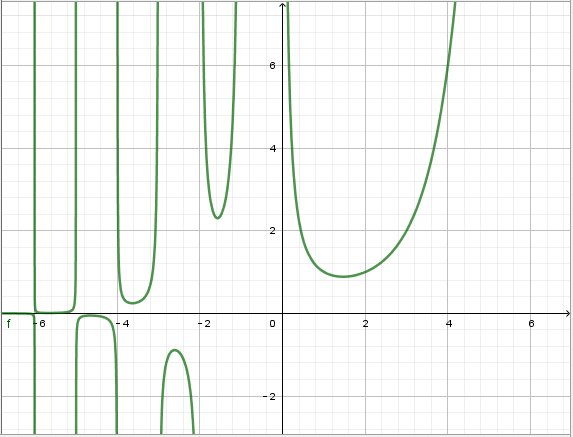
\includegraphics[width=3.5cm]{example.png}
                    \caption{伽马函数示意图}
                \end{wrapfigure}
                答案答案答案答案答案答案答案答案答案答案答案答案答案答案答案答案
                答案答案答案答案答案答案答案答案答案答案答案答案答案答案答案答案
                答案答案答案答案答案答案答案答案答案答案答案答案答案答案答案答案
            \end{minipage}
        \end{solution}
    \end{subquestions}
\end{questions}

\end{document}